\documentclass{beamer}
\usepackage{amsmath, amssymb}
\usepackage{graphicx}
\usepackage{hyperref}
\usepackage{listings}
\usepackage{xcolor}
\usepackage[utf8]{inputenc}

\usetheme{Madrid}
\usecolortheme{default}

\setbeamersize{text margin left=0.8cm}
\setbeamersize{text margin right=0.8cm}
\setbeamersize{sidebar width left=0pt}
\setbeamersize{sidebar width right=0pt}

\title{Probabilistic optimization in manufacturing}
\subtitle{Simulated Annealing meets Set Packing}
\author{Michal Racko \\ PyCon PL 2025}
\date{August 30, 2025}

\lstset{
    language=Python,
    basicstyle=\ttfamily\tiny,
    keywordstyle=\color{blue},
    commentstyle=\color{gray},
    stringstyle=\color{red},
    showstringspaces=false,
    breaklines=false,
    breakatwhitespace=true,
    frame=single,
    frameround=tttt,
    framesep=5pt,
    columns=fullflexible,
    keepspaces=true,
    literate={>>>}{{\textcolor{red}{>\!>\!>}}}3
             {...}{{\textcolor{red}{.\!.\!.}}}3
}

\begin{document}

\begin{frame}
  \titlepage
  \vspace{-0.5cm}
  \begin{center}
    
\includegraphics[width=2.5cm]{images/github.png}
    \\[0.2cm]
    \small{https://github.com/michal-racko/pycon\_pl\_2025}
  \end{center}
\end{frame}

\section{Introduction}

\begin{frame}{What are Monte Carlo methods?}
  \begin{itemize}
    \item Statistical techniques using random sampling
    \item Solve problems that are impossible or impractical to solve analytically
    \item Key principle: Use randomness to approximate deterministic results
  \end{itemize}
  
  \vspace{0.5cm}
  \textbf{Applications:}
  \begin{itemize}
    \item Physics simulations
    \item Financial modeling
    \item Machine learning
    \item Engineering optimization
  \end{itemize}
\end{frame}

\section{Basic concept}

\begin{frame}{Starting at square one}
  \framesubtitle{Value of $\pi$ can be estimated using random sampling}
  \begin{columns}[c]
    \begin{column}{0.5\textwidth}
      Let's pretend $\pi$ is an unknown constant which has to be estimated.
      \vspace{0.5cm}

      \textbf{Geometric considerations}
      \begin{itemize}
        \item Circle area: $A_{circle} = \pi$
        \item Square area: $A_{square} = 4$
        \item Ratio: $\frac{\pi}{4} = \frac{A_{circle}}{A_{square}}$
      \end{itemize}
      
      \vspace{0.5cm}
      Therefore: $\pi = 4 \times \frac{A_{circle}}{A_{square}}$
    \end{column}
    \begin{column}{0.5\textwidth}
      \begin{center}
        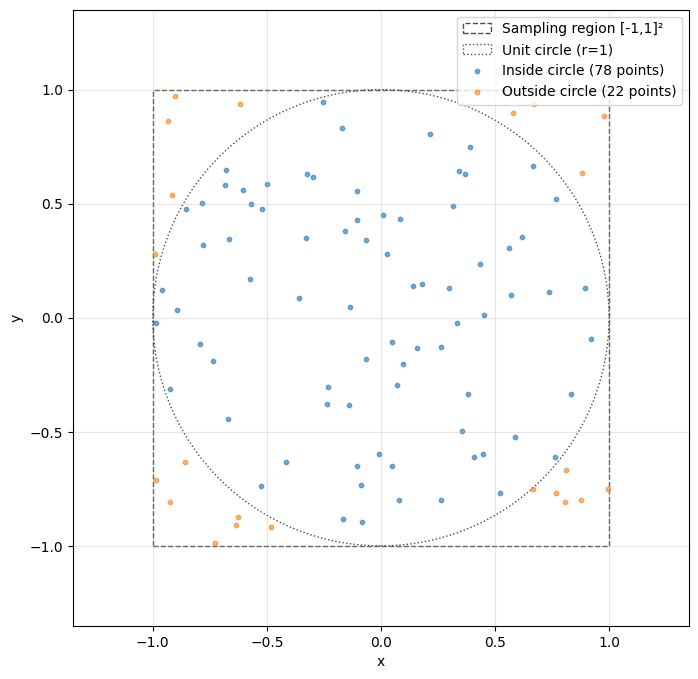
\includegraphics[width=\textwidth]{images/unit_circle_diagram.png}
        \\[0.2cm]
        \small{Unit circle inscribed in square}
      \end{center}
    \end{column}
  \end{columns}
\end{frame}

\begin{frame}{Starting at square one}
  \framesubtitle{Value of $\pi$ can be estimated using random sampling}
  \textbf{Key Insight:} All random points are uniformly distributed in the square

  \begin{itemize}
    \item Point $(x,y)$ is \textcolor{blue}{inside} circle if: $x^2 + y^2 \leq 1$
    \item Point $(x,y)$ is \textcolor{orange}{outside} circle if: $x^2 + y^2 > 1$
  \end{itemize}
  
  \vspace{0.5cm}
  \textbf{Therefore we can estimate}
  $$\pi \approx 4 \times \frac{\text{points inside circle}}{\text{total points}}$$
\end{frame}

\begin{frame}[fragile]{Starting at square one}
  \framesubtitle{Value of $\pi$ can be estimated using random sampling}
\begin{lstlisting}
>>> import numpy as np
>>> class MonteCarloSamples:
...     def __init__(self, n_samples: int):
...         # Generate random points in [-1,1] x [-1,1]
...         self._samples = np.random.random((n_samples, 2)) * 2 - 1
...
...     def __len__(self) -> int:
...         return len(self._samples)
...
...     @property
...     def centre_distances(self) -> np.ndarray:
...         return np.sqrt((self._samples ** 2).sum(axis=1))
...     
...     @property
...     def within_unit_circle(self) -> np.ndarray:
...         return self.centre_distances <= 1
...     
...     @property
...     def pi_estimate(self) -> float:
...         return float(self.within_unit_circle.sum() / len(self) * 4)
...
>>> samples = MonteCarloSamples(100)
>>> print(samples.pi_estimate)
3.12
\end{lstlisting}
\end{frame}

\begin{frame}{Starting at square one}
  \framesubtitle{Value of $\pi$ can be estimated using random sampling}
  \begin{columns}[c]
    \begin{column}{0.5\textwidth}
      Adding more random samples improves precision
      \vspace{0.5cm}

      \textbf{Geometric considerations}
      \begin{itemize}
        \item 100 samples: $\pi \approx 3.12$
        \item 5,000 samples: $\pi \approx 3.1680$
        \item 10,000,000 samples: $\pi \approx 3.1408$
      \end{itemize}
    \end{column}
    \begin{column}{0.5\textwidth}
      \begin{center}
        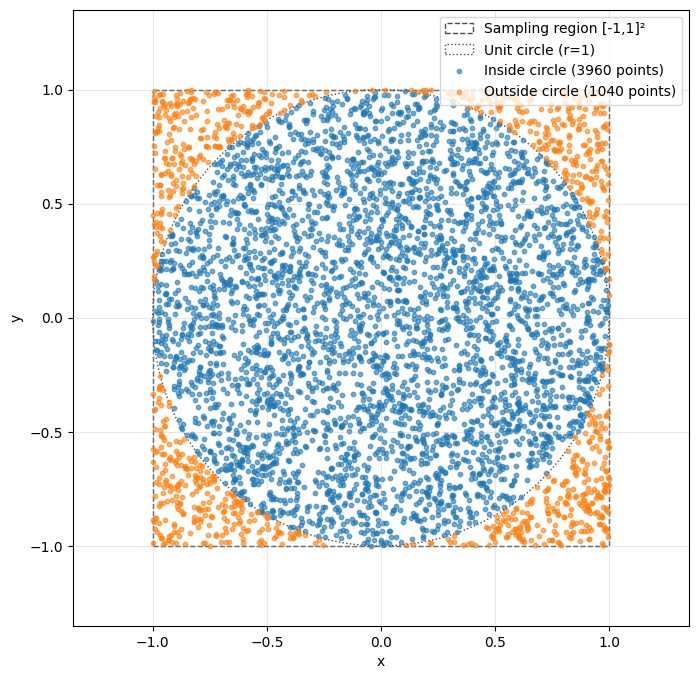
\includegraphics[width=\textwidth]{images/more_samples.png}
        \\[0.2cm]
        \small{More random points drawn from the uniform distribution}
      \end{center}
    \end{column}
  \end{columns}
\end{frame}

\begin{frame}{Starting at square one}
  \framesubtitle{Value of $\pi$ can be estimated using random sampling}

  \begin{columns}[c]
    \begin{column}{0.6\textwidth}
      \begin{center}
        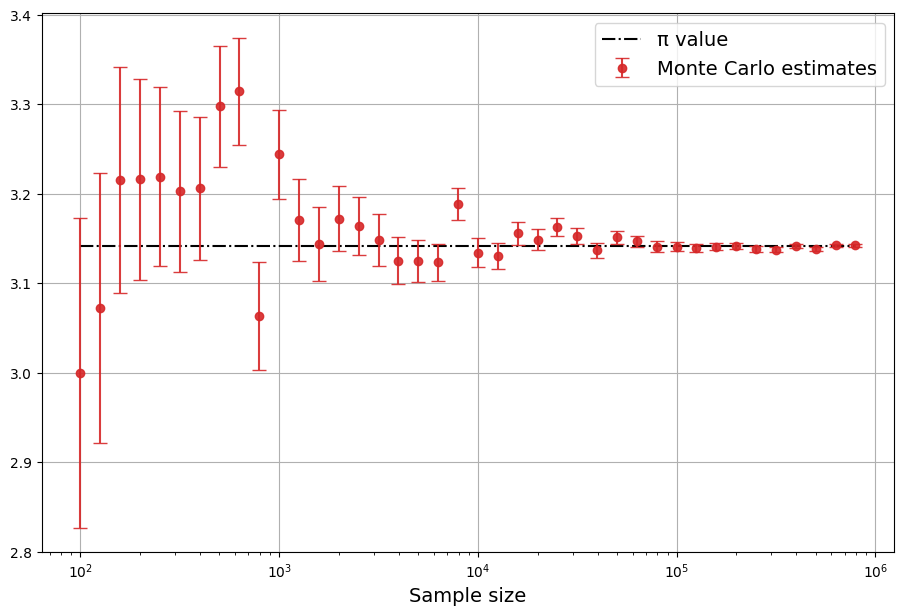
\includegraphics[width=\textwidth]{images/pi_convergence.png}
        \\[0.2cm]
        \small{Monte Carlo estimates converge to the true value as $N \to \infty$}
      \end{center}
    \end{column}
    \begin{column}{0.4\textwidth}
      \textbf{Uncertainty estimation}
      \begin{itemize}
        \item Our estimate follows: $X \sim \text{Binomial}(N, p)$
        \item $\text{Var}(\hat{\pi}) = 16 \cdot \frac{p(1-p)}{N}$
        \item Standard deviation: $\sigma \propto \frac{1}{\sqrt{N}}$
      \end{itemize}
    \end{column}
  \end{columns}
\end{frame}

\begin{frame}[fragile]{Starting at square one}
  \framesubtitle{Value of $\pi$ can be estimated using random sampling}

  \textbf{Estimating via Random Sampling:} Random sampling can estimate quantities
  of interest when the experimental setup is well designed

  \vspace{0.5cm}

  \textbf{Sample Size vs. Error:} Estimation error decreases as sample size grows,
  although larger sample sizes increase computational complexity

  \vspace{0.5cm}

  \textbf{Quantifying Uncertainty:} Uncertainty can be inferred using
  the properties of the probability distribution underlying the random samples

  \vspace{0.5cm}
\end{frame}

\section{Financial Modeling}

\begin{frame}{S\&P 500 price prediction}
  \framesubtitle{Monte Carlo can model complex or poorly understood processes}
  \begin{columns}[c]
    \begin{column}{0.4\textwidth}
      Let's divide and conquer
      \vspace{0.5cm}

      \textbf{Decompose timeseries}
      \begin{itemize}
        \item Exponential Trend: $P_{\text{e}}(t) = a \cdot e^{bt} + c$
        \item Brownian motion: $\Delta P_{\text{b}}(t) = \frac{P(t) - P_{\text{e}}(t)}{P_{\text{e}}(t)}$
      \end{itemize}

      \vspace{0.6cm}
      $P(t) = P_{\text{e}}(t) \times (1 + \Delta P_{\text{b}}(t))$
    \end{column}
    \begin{column}{0.5\textwidth}
      \begin{center}
        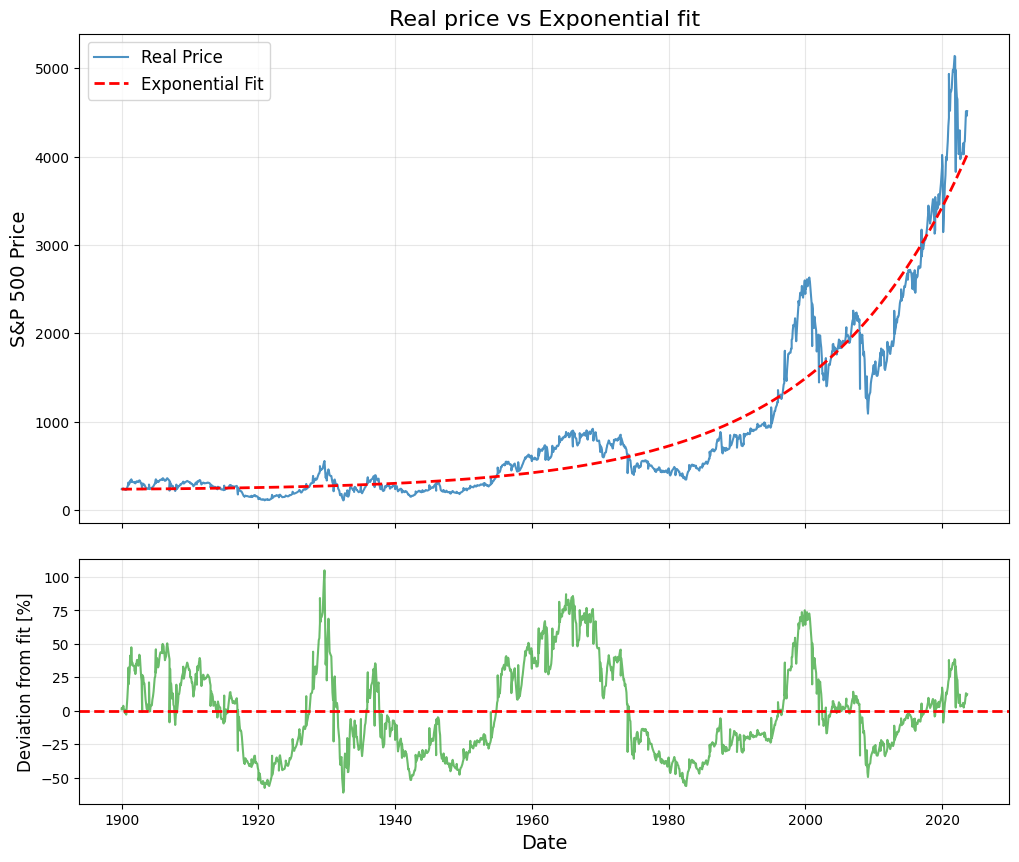
\includegraphics[width=\textwidth]{images/snp500-fit.png}
        \\[0.2cm]
        \small{Exponential growth of S\&P 500}
      \end{center}
    \end{column}
  \end{columns}
\end{frame}

\begin{frame}{S\&P 500 price prediction}
  \framesubtitle{Monte Carlo can model complex or poorly understood processes}

  \textbf{Triple Gaussian mixture:}
  $$f(x) = a_1 \cdot \mathcal{N}(\mu_1, \sigma_1^2) + a_2 \cdot \mathcal{N}(\mu_2, \sigma_2^2) + a_3 \cdot \mathcal{N}(\mu_3, \sigma_3^2)$$

  \begin{columns}[c]
  \begin{column}{0.6\textwidth}
    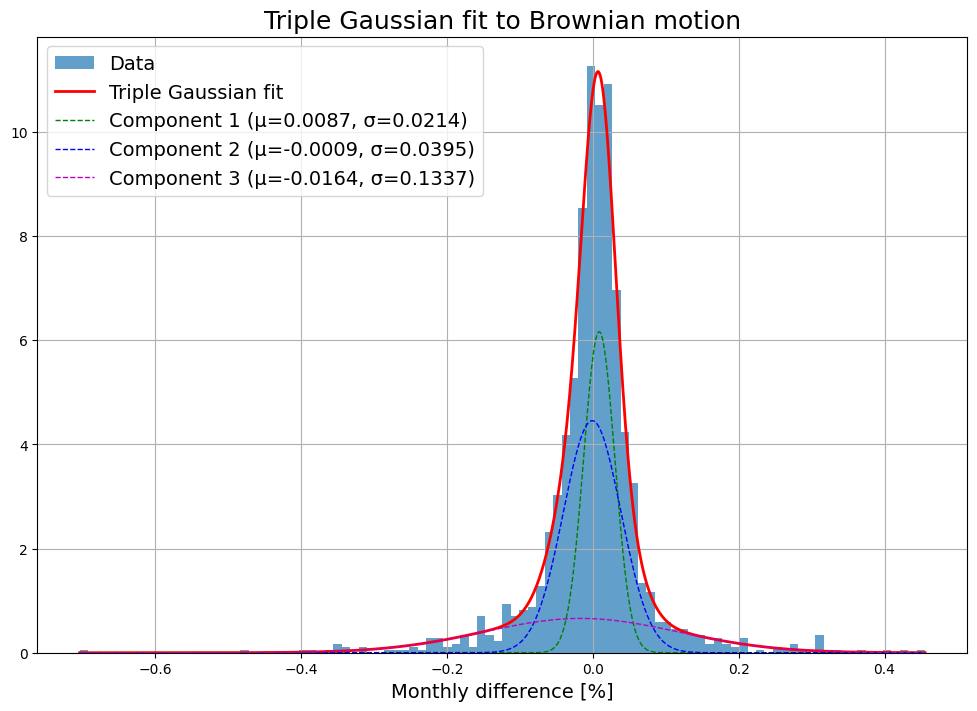
\includegraphics[width=\textwidth]{images/triple_gauss.png}
  \end{column}
  \begin{column}{0.4\textwidth}
    \textbf{Different regimes}
    \begin{itemize}
      \item Normal market conditions
      \item Market stress/crashes
      \item Market euphoria/bubbles
    \end{itemize}
  \end{column}
  \end{columns}
\end{frame}

\begin{frame}[fragile]{S\&P 500 price prediction}
  \framesubtitle{Monte Carlo can model complex or poorly understood processes}

Now draw random samples from the fitted distribution

\vspace{0.5cm}

\begin{lstlisting}
>>> import numpy as np
>>> N_SAMPLES = 10_000
>>> total_weight = a1 + a2 + a3
>>> component_choice = np.random.random(N_SAMPLES)
>>> samples = np.where(
...     component_choice < a1 / total_weight,
...     np.random.normal(mu1, sigma1, N_SAMPLES),
...     np.where(
...         component_choice < (a1 + a2) / total_weight,
...         np.random.normal(mu2, sigma2, N_SAMPLES),
...         np.random.normal(mu3, sigma3, N_SAMPLES)
...     )
... )
>>> samples
array([-0.00252675,  0.15553425,  0.0344586 , ...,  0.01754364,
       -0.01048925, -0.01011193], shape=(10000,))
\end{lstlisting}

\vspace{0.5cm}

and repeat this for every timestep of our simulation\ldots

\end{frame}

\begin{frame}{S\&P 500 price prediction}
  \framesubtitle{Monte Carlo can model complex or poorly understood processes}
  \begin{columns}[c]
    \begin{column}{0.4\textwidth}
      \textbf{Many experiments}
      \begin{itemize}
        \item Every simulated path represents an alternative reality following the same principles as our real data
        \item The more paths in a given region the more likely it is to occur
        \item Variance reduction techniques help focus on important regions
      \end{itemize}
    \end{column}
    \begin{column}{0.6\textwidth}
      \begin{center}
        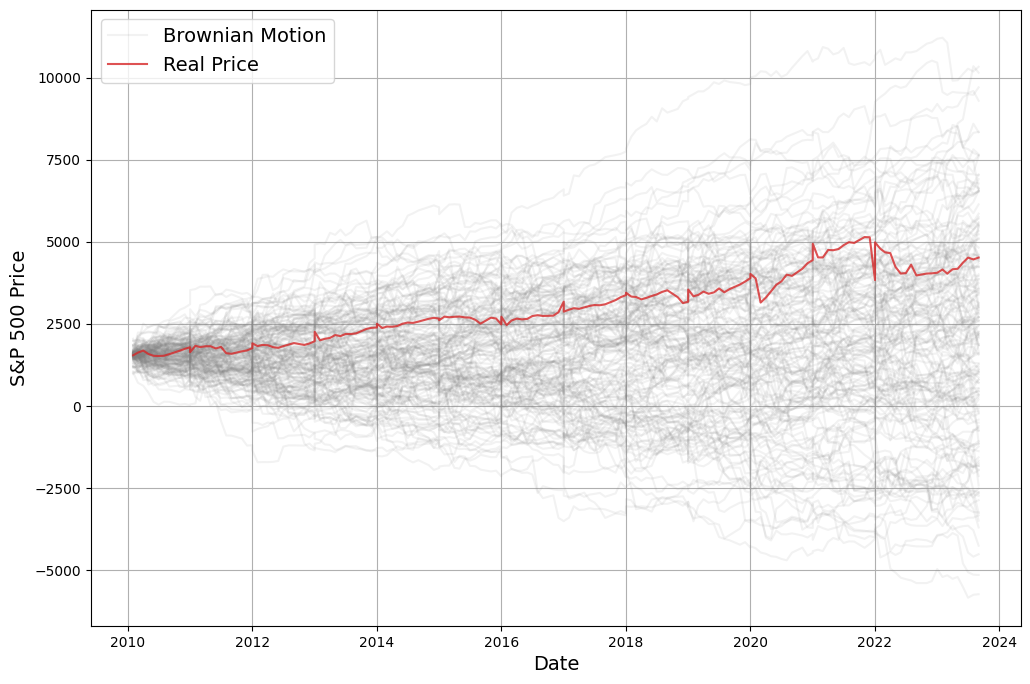
\includegraphics[width=\textwidth]{images/brownian_paths.png}
        \\[0.2cm]
        \small{Simulated S\&P 500 paths}
      \end{center}
    \end{column}
  \end{columns}
\end{frame}

\begin{frame}{S\&P 500 price prediction}
  \framesubtitle{Monte Carlo can model complex or poorly understood processes}
  \begin{columns}[c]
    \begin{column}{0.5\textwidth}
      \begin{center}
        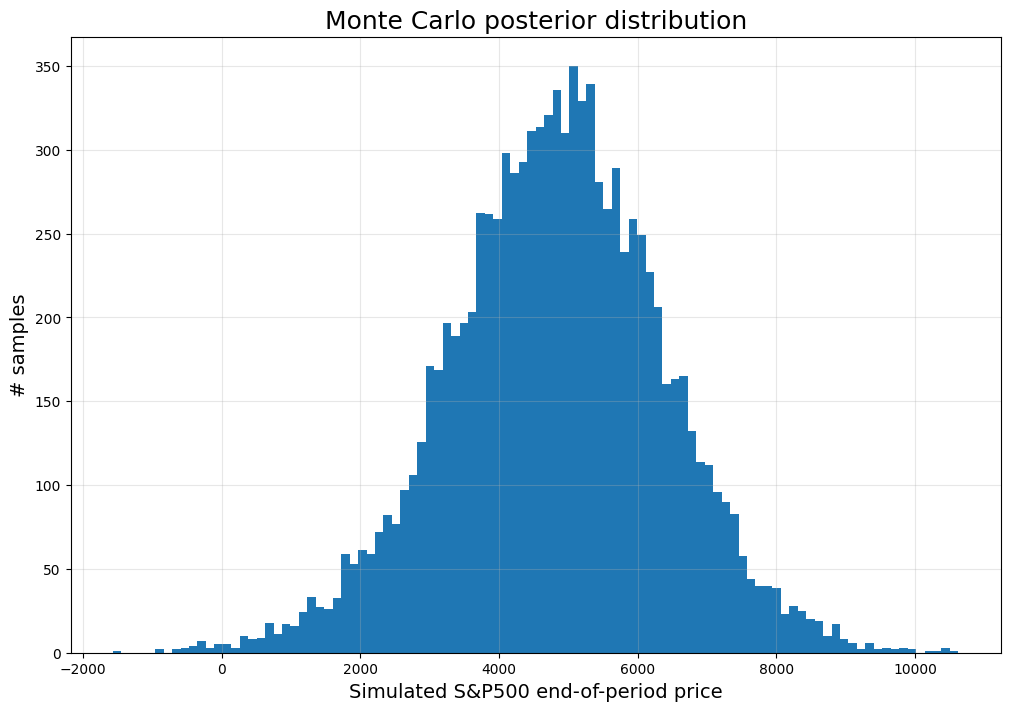
\includegraphics[width=\textwidth]{images/posterior.png}
        \\[0.2cm]
        \small{Monte Carlo posterior comprises results from all parallel experiments}
      \end{center}
    \end{column}
    \begin{column}{0.5\textwidth}
      \textbf{Our simulation}
      \begin{itemize}
        \item Gives probability estimates for future outcomes
        \item Past two years gets a Z-score of 1.0444
        \item While this model is rather simplistic it still provides useful insights
      \end{itemize}
    \end{column}
  \end{columns}
\end{frame}

\begin{frame}{S\&P 500 price prediction}
  \framesubtitle{Monte Carlo can model complex or poorly understood processes}

  \textbf{Modeling with Monte Carlo:} Complex or poorly understood processes
  can be modeled using random distributions, which Monte Carlo methods then
  leverage to simulate possible future outcomes

  \vspace{0.5cm}

  \textbf{Assessing Future Outcomes:} Posterior distributions allow us to
  estimate the likelihood of future outcomes, providing a powerful tool
  for assessing risks and opportunities

  \vspace{0.5cm}

  \textbf{Statistical Weight Implementation:} Variance reduction techniques
  allow our model to concentrate computational effort on the most important
  regions of the outcome space

  \vspace{0.5cm}
\end{frame}

\section{Probabilistic optimization}

\begin{frame}{Probabilistic optimization}
  \framesubtitle{Simulated Annealing escapes local optima}
  \begin{columns}[c]
    \begin{column}{0.4\textwidth}
      \textbf{The Challenge:} Roadtrip around Poland
      \vspace{0.5cm}

      \textbf{Problem complexity}
      \begin{itemize}
        \item NP-hard optimization problem
        \item $(n-1)!/2$ possible routes for n cities
        \item 21 cities $\to$ $\sim10^{18}$ combinations
      \end{itemize}
    \end{column}
    \begin{column}{0.6\textwidth}
      \begin{center}
        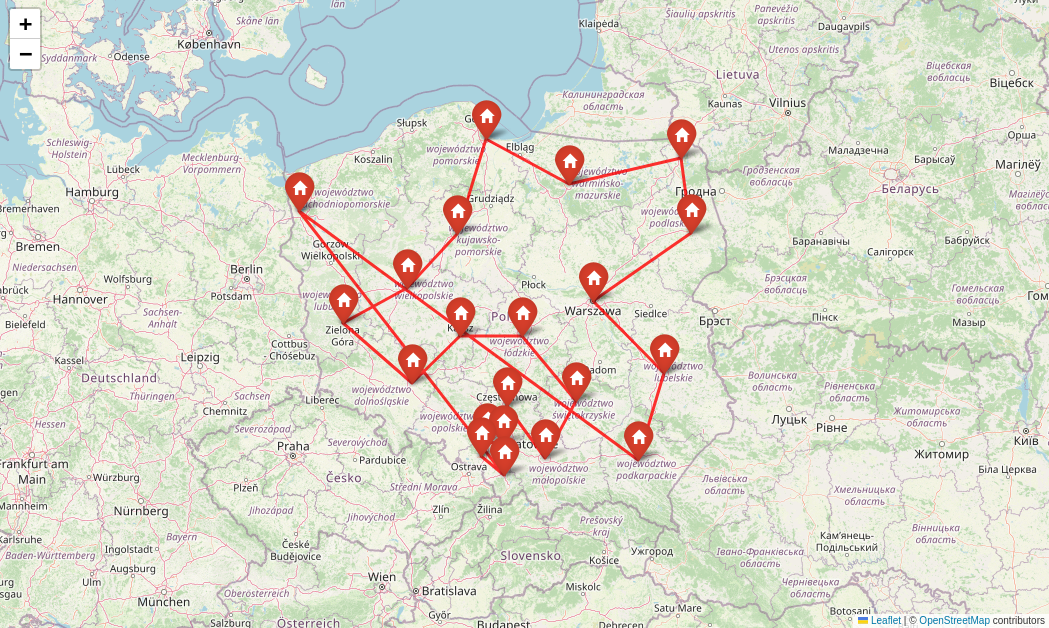
\includegraphics[width=\textwidth]{images/tsp-naive.png}
        \\[0.2cm]
        \small{Naive solution to TSP gets trapped in a local minimum}
      \end{center}
    \end{column}
  \end{columns}
\end{frame}

\begin{frame}{Probabilistic optimization}
  \framesubtitle{Simulated Annealing escapes local optima}

  \begin{columns}[c]
    \begin{column}{0.4\textwidth}
      \textbf{Common for:}

      \begin{itemize}
        \item Sheet metal production
        \item Quartz minerals
        \item Nuclear energy
      \end{itemize}

      \vspace{0.5cm}

      \textbf{Boltzmann Distribution:}
      $$P(E) \propto e^{-\frac{E}{k_B T}}$$

      \textbf{Simulated analogy:}
    \end{column}
    \begin{column}{0.6\textwidth}
      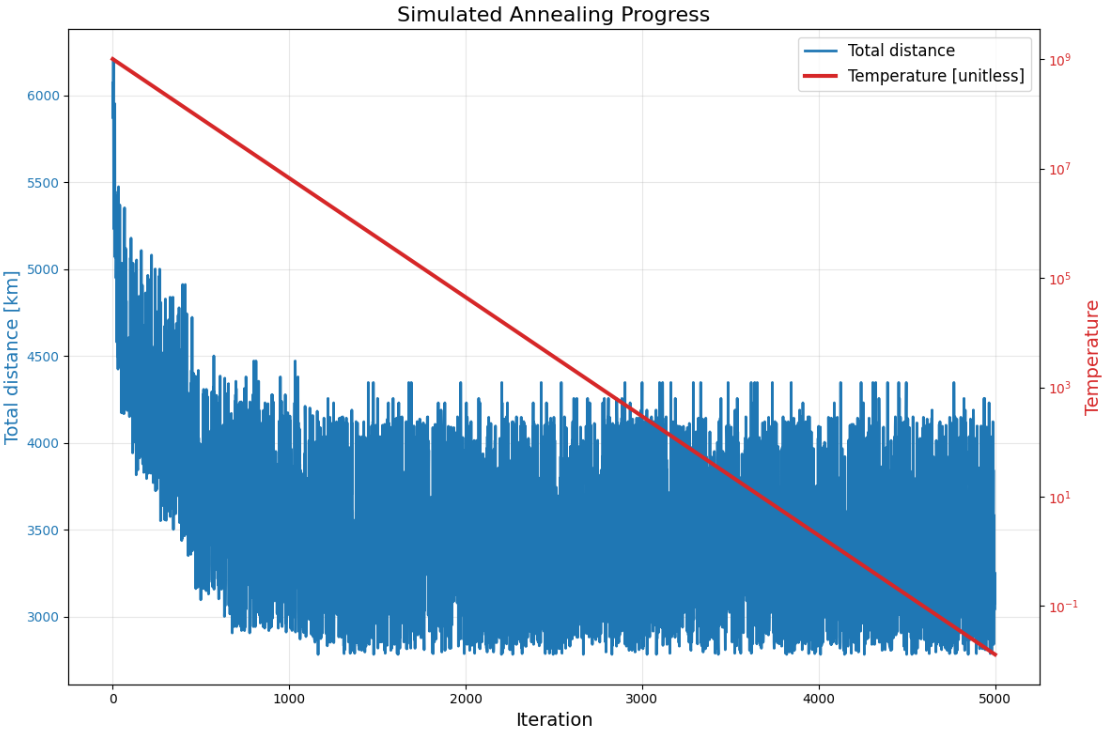
\includegraphics[width=\textwidth]{images/annealing-history.png}
    \end{column}
  \end{columns}

  \vspace{0.5cm}

  $$P(\text{accept worse solution}) = e^{-\frac{\text{distance increase}}{T}}$$
\end{frame}

\begin{frame}{Probabilistic optimization}
  \framesubtitle{Simulated Annealing escapes local optima}
  \begin{columns}[c]
    \begin{column}{0.4\textwidth}
      \textbf{Algorithm}
      \begin{itemize}
        \item \textbf{Exploration phase} high T $\Rightarrow$ most moves are accepted
        \item \textbf{Exploitation phase} low T $\Rightarrow$ only improvements are accepted
      \end{itemize}

      \textbf{My implementation}
      Batch annealing plant optimization
    \end{column}
    \begin{column}{0.6\textwidth}
      \begin{center}
        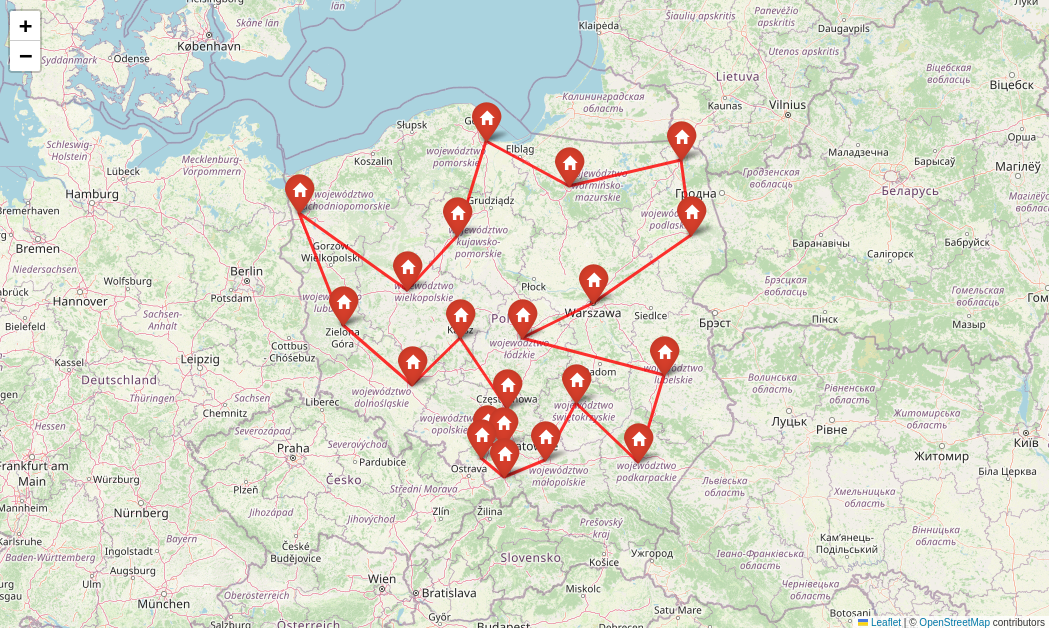
\includegraphics[width=\textwidth]{images/tsp-annealing.png}
        \\[0.2cm]
        \small{Simulated annealing finds approximation to the optimal solution}
      \end{center}
    \end{column}
  \end{columns}
\end{frame}

\begin{frame}{Probabilistic optimization}
  \framesubtitle{Simulated Annealing escapes local optima}

  \textbf{Monte Carlo in Optimization:} Randomness enables exploration of solution
  spaces that deterministic algorithms cannot effectively navigate

  \vspace{0.5cm}

  \textbf{Temperature Scheduling:} Controlled cooling balances exploration
  (high temperature) with exploitation (low temperature) to find global optima

  \vspace{0.5cm}

  \textbf{Real-world Impact:} TSP principles apply to logistics, manufacturing,
  and many more\ldots

  \vspace{0.5cm}
\end{frame}

\begin{frame}{Thank You!}
  \begin{center}
    \Large{I'm looking forward to answering your questions}
  \end{center}
\end{frame}

\end{document}